\documentclass[12pt,a4paper]{beamer}
\usepackage{setspace}
\usepackage[utf8x,utf8]{inputenc}
\usepackage[ngerman]{babel}
\usepackage{ucs}
\usepackage{amsmath}
\usepackage{amsfonts}
\usepackage{amssymb}
\usepackage{lmodern}
\usepackage{hyperref}

% Beamer Settings
\usetheme{Singapore}

% Default Presentation Settings
\title{Remote Logging mit rsyslog}
\subtitle{Inklusive Tools zur Überwachung und Verwaltung}
\author{Thomas Merkel \and Arkadiusz Rawa \and Janik Lemcke}
\institute{Hochschule Ravensburg-Weingarten}
\date{\today} 

\begin{document}
	% Intro
	\begin{frame}
		\titlepage
	\end{frame} 
	\begin{frame}
		\tableofcontents
	\end{frame}
	
	% Presentation Parts
	\section{Remote Logging}
\subsection{Problem}
\begin{frame}[plain]
	\frametitle{Remote Logging}
	\framesubtitle{Problem}
	\begin{center}
		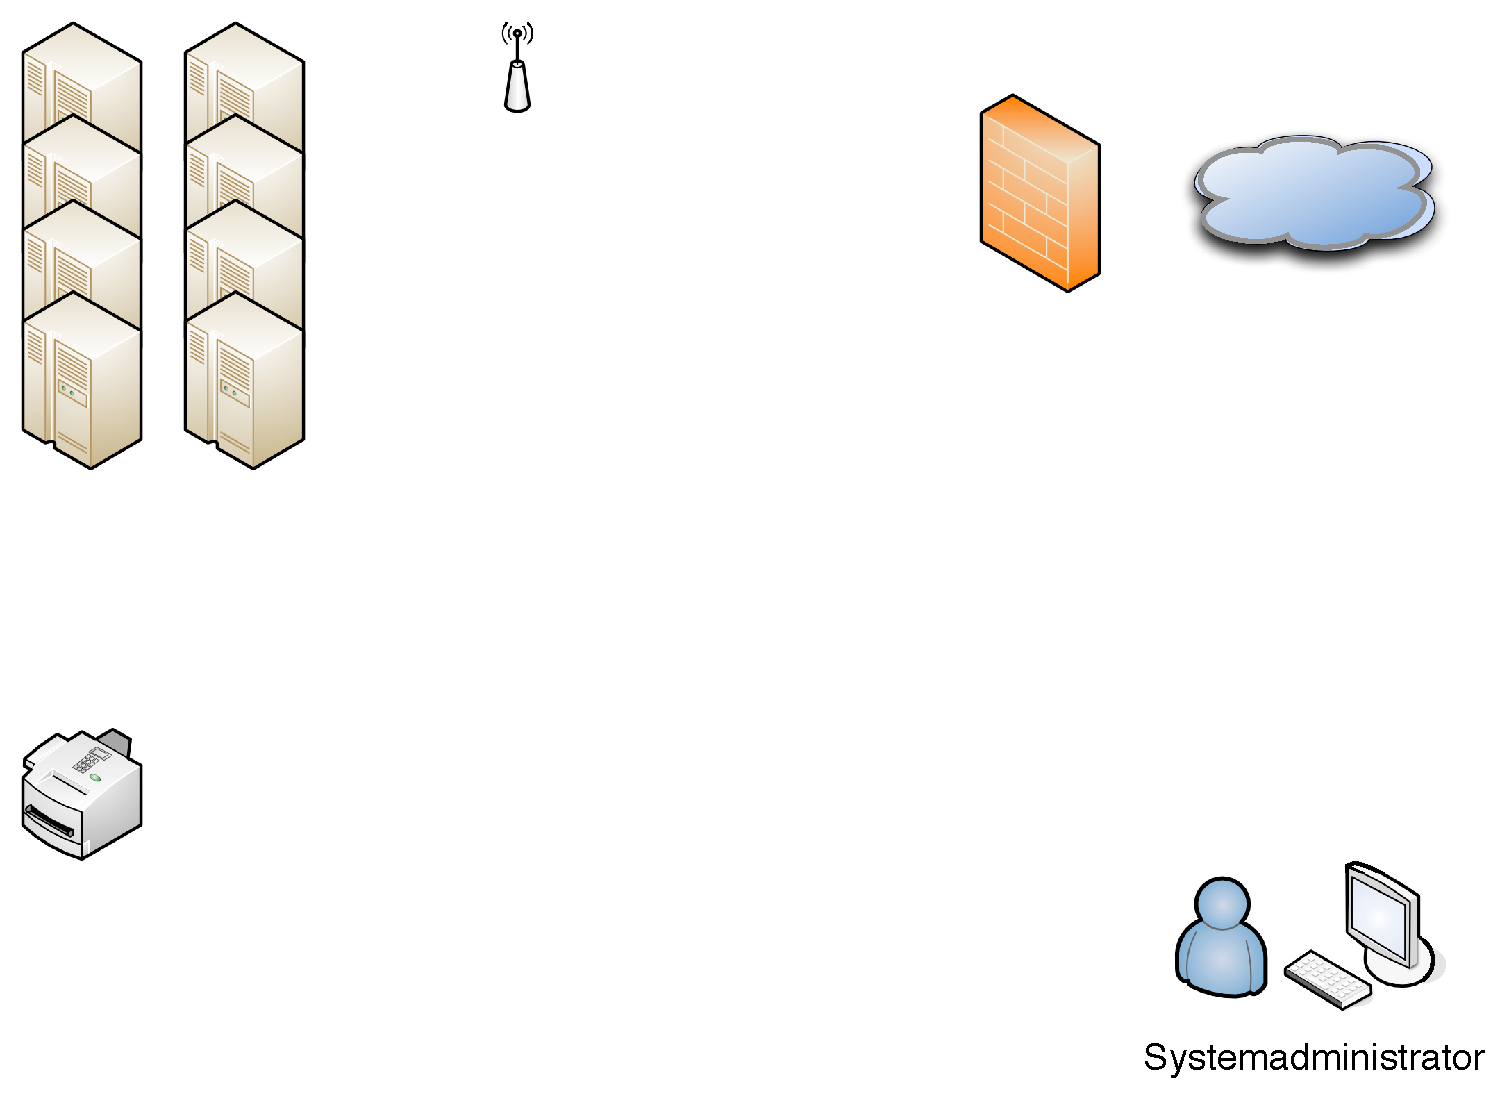
\includegraphics[width=\linewidth]{images/remote_logging_01.eps}
	\end{center}
\end{frame}

\subsection{Panic}
\begin{frame}[plain]
	\frametitle{Remote Logging}
	\framesubtitle{Panic}
	\begin{center}
		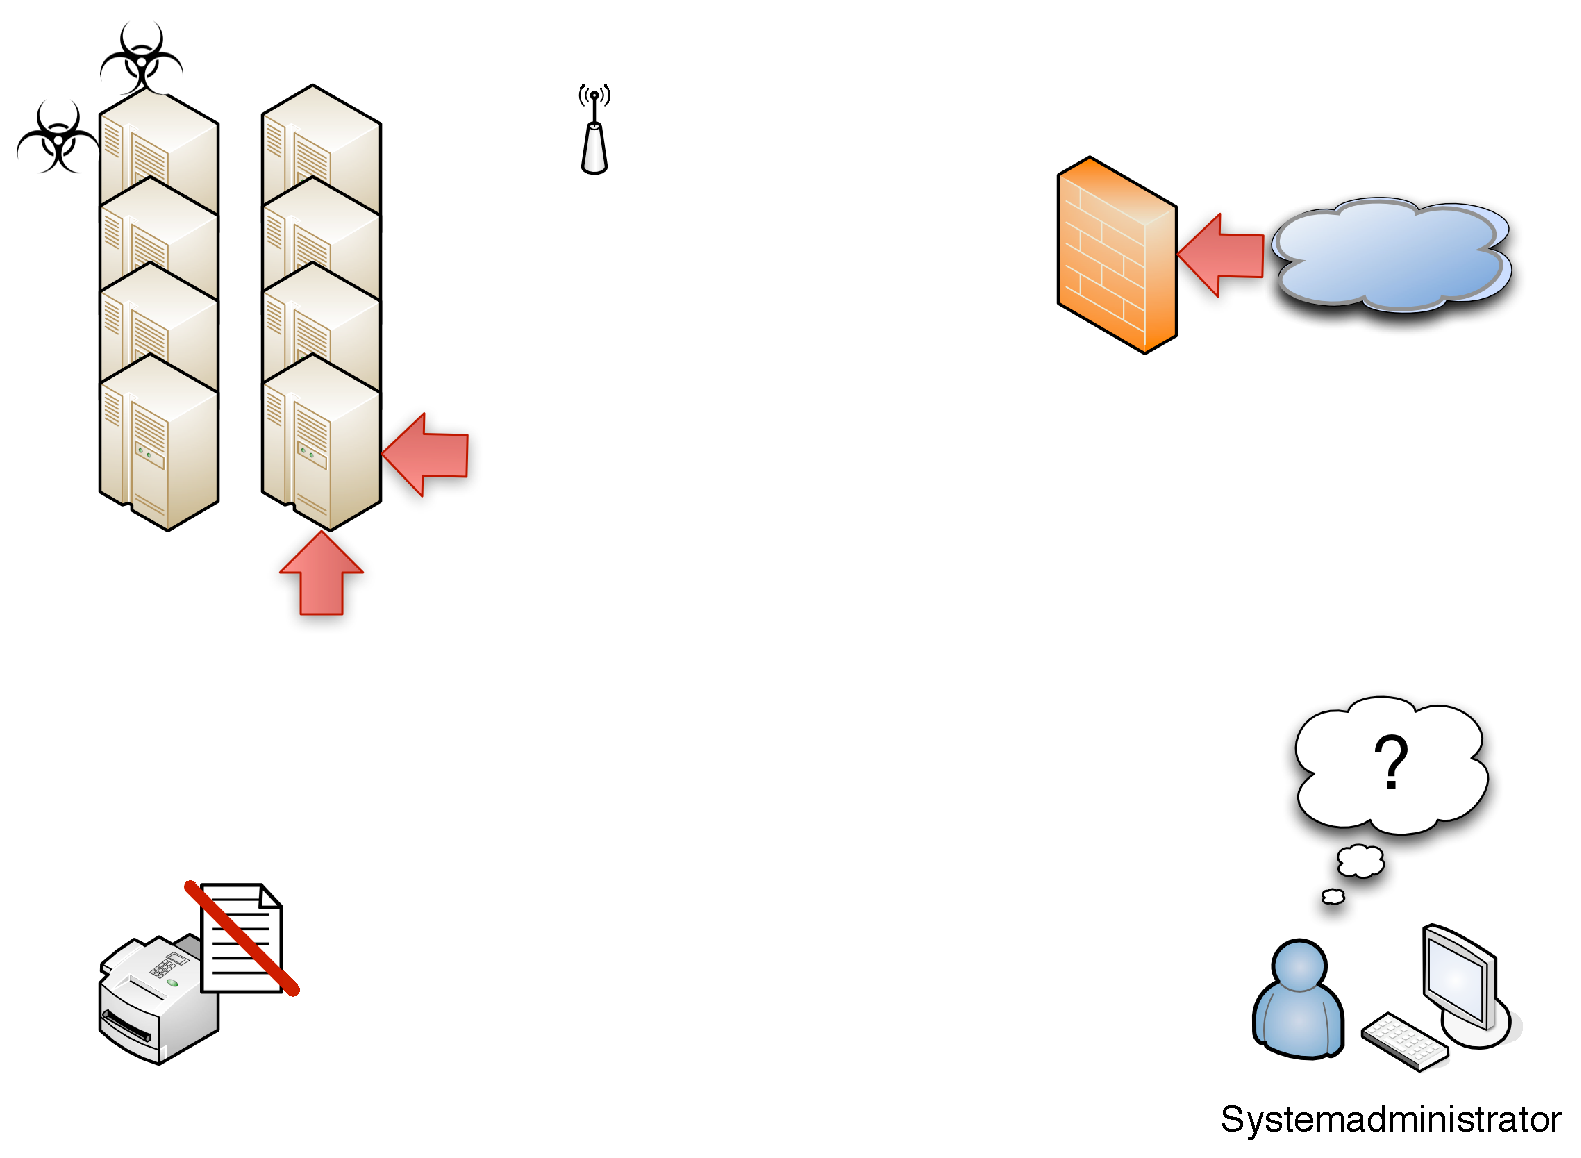
\includegraphics[width=\linewidth]{images/remote_logging_02.eps}
	\end{center}
\end{frame}

\subsection{Don't Panic}
\begin{frame}[plain]
	\frametitle{Remote Logging}
	\framesubtitle{Don't Panic}
	\begin{center}
		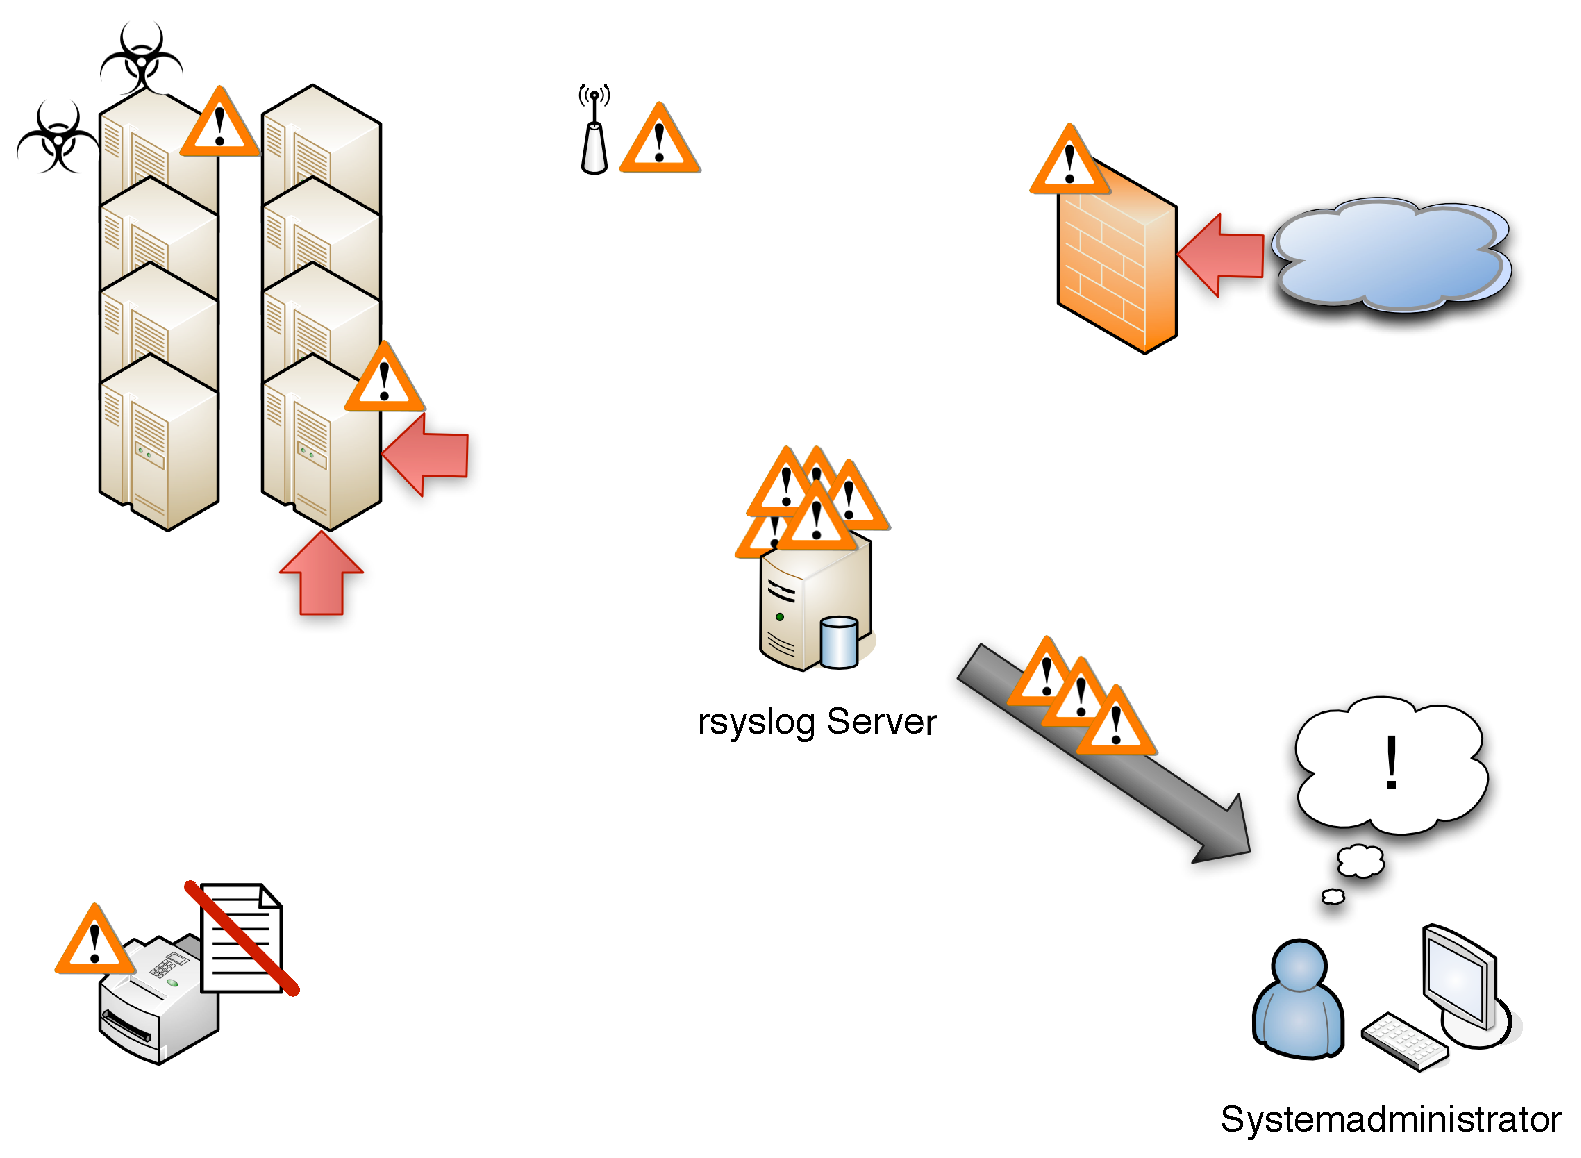
\includegraphics[width=\linewidth]{images/remote_logging_03.eps}
	\end{center}
\end{frame}

\subsection{Ziele}
\begin{frame}
	\frametitle{Remote Logging}
	\framesubtitle{Ziele}
	\begin{itemize}
		\item Alle Informationen an einem zentralen System
		\item Archivierung ist zentralisiert
		\item Alarmierung
		\item Monitoring
	\end{itemize}
\end{frame}
	\section{rsyslog}
	\subsection{Überblick}
		Rsyslog ist ein weiterer syslog-Daemon für Linux beziehungsweise Unix-Systeme. Er bietet, durch 
		die Möglichkeit der inhaltsbasierten Filterung, eine gute Grundlage für jedes System.
		In diesem Abschnitt wird die Installation und Konfiguration von rsyslog für den Remote Logging
		Einsatz vorgestellt.

		\Hinweisbox{
			Es wird rsyslog in der Version 4.6.4-2 unter Ubuntu Server 10.04 LTS eingesetzt. 
			Die Konfiguration kann daher unter anderen Versionen und Distributionen abweichen.
		}

	\subsection{Alternativen}
		Um einen besseren Überblick über die syslog-Landschaft zu erhalten werden einige Alternativen vorgestellt.
		\subsubsection*{syslogd}
		Bei syslogd handelt es sich um den ältesten und bekanntesten Protokoll-Daemon.\cite{GentooProtokollierung}
		\subsubsection*{syslog-ng}
	\subsection{Remote logging}
		\subsubsection*{Vorteile}
		\subsubsection*{Nachteile}
	\subsection{Installation}
		In einigen Linux Distributionen wie zum Beispiel Debian und Ubuntu ist rsyslog schon zum Standard 
		geworden. Für andere Distributionen empfiehlt es sich den Paketmanager zur Installation zu verwenden.

		\begin{tabular}{ll}
			\hline
			Linux Distribution & Installationsbefehl\\
			\hline\hline
			Debian, Ubuntu & apt-get install rsyslog\\
			SUSE, openSUSE & yast -i rsyslog\\
			Fedora         & yum install rsyslog\\
			Gentoo         & emerge rsyslog
		\end{tabular}

		\Hinweisbox{
			Gentoo Benutzer sollten die passenden Useflags für das rsyslog Paket beachten. Empfehlenswert sind
			\textit{gnutls}, \textit{logrotate} und \textit{zlib}. 
		}

	\subsection{Konfiguration}
		\subsubsection*{Server}
		\subsubsection*{Linux Client}
		\subsubsection*{Windows Client}
		\subsubsection*{Debugging}


	\section{tenshi}
\begin{frame}
	\frametitle{tenshi}
	\framesubtitle{Allgemeines}
	bla bla
\end{frame}
	\section{phpLogCon}
\subsection{Überblick}
\begin{frame}
	\frametitle{phpLogCon}
	\framesubtitle{"Uberblick}
	\begin{itemize}
		\item php-Webinterface mit MySql-Datenbank
		\item tabellarische Darstellung
		\item personalsierbare Ansichten und Filterungen
		\item Diagrammauswertung für besseren Überblick
	\end{itemize}
\end{frame}

\subsection{Installation}
\begin{frame}[fragile]
	\frametitle{phpLogCon}
	\framesubtitle{Installation}
	Die Installation ist so nur unter Ubuntu möglich
	\begin{block}{Debian, Ubuntu}
	\begin{verbatim}
		Lamp Server
		apt-get install rsyslog-mysql
		apt-get install rsyslog-relp
	\end{verbatim}
	\end{block}
\end{frame}

\subsection{Webinterface}
\begin{frame}
	\frametitle{phpLogCon}
	\framesubtitle{Webinterface}
	\begin{itemize}
		\item Suche
		\item Meldungen
		\item Statistiken
		\item Administration
	\end{itemize}
\end{frame}

\subsubsection{Suche}
\begin{frame}
	\frametitle{phpLogCon - Webinterface}
	\framesubtitle{Suche}
	\begin{center}
		\includegraphics[width=\linewidth]{images/phplogcon_suche.eps}
	\end{center}
\end{frame}

\subsubsection{Meldungen}
\begin{frame}
	\frametitle{phpLogCon - Webinterface}
	\framesubtitle{Meldungen}
	\begin{center}
		\includegraphics[width=\linewidth]{images/phplogcon_meldungen.eps}
	\end{center}
\end{frame}

\subsubsection{Statistiken}
\begin{frame}
	\frametitle{phpLogCon - Webinterface}
	\framesubtitle{Statistiken}
	\begin{center}
		\includegraphics[width=\linewidth]{images/phplogcon_statistik.eps}
	\end{center}
\end{frame}

\subsubsection{Administration}
\begin{frame}
	\frametitle{phpLogCon - Webinterface}
	\framesubtitle{Administration}
	\begin{center}
	 	\includegraphics[width=\linewidth]{images/phplogcon_admin.eps}
	\end{center}
\end{frame}

\subsection{Alternativen}
\begin{frame}
	\frametitle{phpLogCon}
	\framesubtitle{Alternative: Logzilla}
	\begin{itemize}
		\item Vollinstallation inkl. Betriebssystem
		\item Mehr Möglichkeiten der Analyse
		\item Zusätzliche Funktionen integriert
		\item Shareware, direkter Support möglich
	\end{itemize}
\end{frame}

	% Last Slide
	\section{Diskussion}
	\begin{frame}
		\frametitle{Diskussion}
		\framesubtitle{Fragen, Anregungen, Wünsche}
		\begin{itemize}
			\item Workshop am nächsten Termin der Linux User Group Weingarten
			\item Alle Unterlagen unter \url{https://github.com/drscream/rsyslog-workshop}		
		\end{itemize}
		\bigskip
		\bigskip
		\scriptsize{
			Danke an Paul Nijjar für seine Präsentation: \linebreak 
			\textit{Remote Logging with Rsyslog - How I Learned to Start Worrying and Love the Panopticon}
		}
	\end{frame}
\end{document}